\chapter{Rangkaian Arus Searah: Hukum dan Teorema Kirchhoff}\label{ch:b1:dc-circuits}

Putarlah kunci kontak pada pagi yang dingin: motor starternya
menggeram, lampu dasbornya meredup sesaat, lalu mobilnya terbatuk hidup.
Aki yang sesaat tadi memberi \qty{12.6}{V} yang mantap kini turun ke
sebelas volt selagi starternya menarik seratus lima puluh \omterm{def:b1:dc-circuits:current}{ampere} --- dan
lampu depannya, yang terpasang paralel, ikut membayarnya. Segala hal
dalam sekon itu diatur oleh dua hukum kekekalan dan sejumlah kecil
teorema tentang \omterm{def:b1:dc-circuits:linear}{rangkaian linear}, yang dinyatakan, dibuktikan dan
diterapkan bab ini: \omterm{thm:b1:dc-circuits:kirchhoff}{hukum Kirchhoff}, model sumber dan \omterm{def:b1:dc-circuits:resistor}{resistor}, pembagi,
Thévenin dan Norton, serta seni grafis mencari \omterm{met:b1:dc-circuits:loadline}{titik kerja}.

\section{Arus, tegangan, dan rezim kuasi-tunak}

\begin{definition}[Arus listrik]\label{def:b1:dc-circuits:current}
\index{arus listrik}\index{ampere}
\emph{Arus listrik} yang melalui sebuah permukaan (penampang lintang
sebuah kawat) adalah muatan yang menyeberanginya tiap satuan waktu,
dihitung positif menurut arah yang dipilih:
\[
i = \frac{\dd q}{\dd t} \qquad (\text{ampere: } \qty{1}{A} = \qty{1}{C/s}).
\]
Membalik arahnya mengubah tanda $i$. Di dalam logam pembawa muatannya
adalah elektron, yang menghanyut \emph{berlawanan} dengan arah arus
konvensionalnya, dengan laju sepersekian milimeter tiap sekon.
\end{definition}

\begin{definition}[Potensial dan tegangan]\label{def:b1:dc-circuits:voltage}
\index{potensial listrik}\index{tegangan}\index{titik tanah}
Setiap titik sebuah rangkaian mempunyai \emph{potensial listrik} $V$
(volt), yang terdefinisi sampai pada suatu tetapan yang ditetapkan
dengan memilih sebuah \emph{titik tanah} ($V = 0$). \emph{Tegangan}
antara $A$ dan $B$ adalah beda potensial $u_{AB} = V_A - V_B$, yang
digambar sebagai anak panah dari $B$ ke $A$. Energi yang dilepaskan
muatan $q$ ketika berjalan dari $A$ ke $B$ adalah $q\,u_{AB}$ (ini
bersambung ke potensial elektrostatik \cref{ch:b1:potential-capacitors}).
\end{definition}

\begin{definition}[Rezim kuasi-tunak (ARQS)]\label{def:b1:dc-circuits:arqs}
\index{rezim kuasi-tunak}\index{ARQS}
Rangkaian berukuran $\ell$ yang digerakkan pada frekuensi $f$ berada
dalam \emph{rezim kuasi-tunak} bila waktu rambat $\ell/c$ \omterm{def:b1:wave-propagation:signal}{sinyal}
listrik di sepanjangnya dapat diabaikan terhadap periodenya $1/f$:
$\ell \ll c/f$. Arusnya lalu sama di setiap titik kawat tak bercabang
pada tiap saat, dan hukum di bawah ini berlaku pada tiap saat bagi arus
dan \omterm{def:b1:dc-circuits:voltage}{tegangan} yang berubah terhadap waktu (huruf kecil $i$, $u$) persis
seperti bagi yang tunak ($I$, $U$).
\end{definition}

\begin{example}[Sekuasi apa kuasi itu]\label{ex:b1:dc-circuits:arqs}
Pada \qty{50}{Hz}, $c/f = \qty{6000}{km}$: sebuah rumah berada dalam
\omterm{def:b1:dc-circuits:arqs}{rezim kuasi-tunak}. Pada \qty{1}{MHz}, \qty{300}{m}: sebuah radio pun
masih. Pada \qty{2}{GHz}, \qty{15}{cm}: papan rangkaian sebuah telepon
tidak, dan jalurnya harus diperlakukan sebagai saluran transmisi ---
sebuah pokok bahasan volume Tahun ke-2.
\end{example}

\begin{theorem}[Hukum Kirchhoff]\label{thm:b1:dc-circuits:kirchhoff}
\index{hukum Kirchhoff}\index{hukum simpul}\index{hukum loop}
Dalam \omterm{def:b1:dc-circuits:arqs}{rezim kuasi-tunak}:
\begin{enumerate}
  \item \emph{\omterm{thm:b1:dc-circuits:kirchhoff}{Hukum simpul}}: pada simpul tempat beberapa kawat bertemu,
        jumlah arus yang tiba sama dengan jumlah arus yang pergi,
        $\sum_{\text{masuk}} i_k = \sum_{\text{keluar}} i_k$.
  \item \emph{\omterm{thm:b1:dc-circuits:kirchhoff}{Hukum loop}}: mengelilingi sebarang loop tertutup, \omterm{def:b1:dc-circuits:voltage}{tegangan}
        berjumlah nol bila dihitung dengan tanda yang diberikan arah
        penelusuran yang dipilih: $\sum_{\text{loop}} \pm u_k = 0$.
\end{enumerate}
\end{theorem}

\begin{proof}
Muatan bersifat kekal dan, dalam \omterm{def:b1:dc-circuits:arqs}{rezim kuasi-tunak}, tidak menumpuk di
sebuah simpul: apa yang tiba tiap sekon pergi tiap sekon pula. \omterm{thm:b1:dc-circuits:kirchhoff}{Hukum
loopnya} adalah pernyataan bahwa potensialnya merupakan fungsi
kedudukan: setelah mengelilingi sebuah loop dan kembali ke titik
awalnya, jumlah penurunan potensialnya adalah $V_A - V_A = 0$.
\end{proof}

\begin{notation}[Kesepakatan dan daya]\label{not:b1:dc-circuits:conventions}
\index{kesepakatan penerima}\index{kesepakatan pembangkit}\index{daya listrik}
Untuk komponen berdua ujung (sebuah \emph{dipol}), \emph{\omterm{thm:b1:dc-circuits:kirchhoff}{kesepakatan
penerima}} menggambar anak panah \omterm{def:b1:dc-circuits:voltage}{tegangan} dan anak panah arus dengan arah
berlawanan; \emph{\omterm{thm:b1:dc-circuits:kirchhoff}{kesepakatan pembangkit}} menggambar keduanya searah.
Dalam \omterm{thm:b1:dc-circuits:kirchhoff}{kesepakatan penerima}, daya yang \emph{diterima} dipolnya adalah
\[
p = u\,i \qquad (\text{watt}),
\]
positif bagi \omterm{def:b1:dc-circuits:resistor}{resistor} yang memanas, negatif bagi baterai yang memberi.
Dalam \omterm{thm:b1:dc-circuits:kirchhoff}{kesepakatan pembangkit}, $p = ui$ adalah daya yang
\emph{diberikan}.
\end{notation}

\begin{omfigure}
\begin{tikzpicture}[font=\small]
  \draw (0,0) to[generic, l=dipol, v=$u$, i=$i$] (3,0);
  \node[below] at (1.5,-1.0) {kesepakatan penerima: $p_{\text{diterima}} = ui$};
  \begin{scope}[xshift=6cm]
  \draw (0,0) to[generic, l=dipol, v<=$u$, i=$i$] (3,0);
  \node[below] at (1.5,-1.0) {kesepakatan pembangkit: $p_{\text{diberikan}} = ui$};
  \end{scope}
\end{tikzpicture}

{\small Dua kesepakatan tanda untuk sebuah dipol: anak panah berlawanan
(penerima) atau searah (pembangkit). Fisikanya sama; hanya tanda $ui$
yang dibacanya berbeda.}
\end{omfigure}

\section{Dipol dan modelnya}

\begin{definition}[Karakteristik; resistor; hukum Ohm]\label{def:b1:dc-circuits:resistor}
\index{karakteristik (dipol)}\index{resistor}\index{hukum Ohm}\index{efek Joule}
\emph{Karakteristik} sebuah dipol adalah kurva $i(u)$ (atau $u(i)$)
yang dipaksakannya. Sebuah \emph{resistor} berkarakteristik linear yang
melalui titik asal, yaitu \emph{hukum Ohm}
\[
u = R\,i \qquad (\text{kesepakatan penerima}),
\]
dengan $R$ sebagai \emph{hambatan}nya (ohm, $\qty{1}{\ohm} = \qty{1}{V/A}$) dan
$G = 1/R$ sebagai \emph{konduktansi}nya (siemens). Ia menerima $p = Ri^2 =
u^2/R \geq 0$, yang dilesapkan sebagai kalor (\emph{efek Joule}). Kawat
sepanjang $\ell$, berpenampang $S$ dan berhambatan jenis $\rho$
mempunyai $R = \rho\ell/S$.
\end{definition}

\begin{definition}[Sumber ideal dan sumber nyata]\label{def:b1:dc-circuits:sources}
\index{sumber tegangan}\index{sumber arus}\index{gaya gerak listrik}\index{hambatan dalam}\index{model Thevenin@model Thévenin}\index{model Norton}
\emph{Sumber \omterm{def:b1:dc-circuits:voltage}{tegangan} ideal} memaksakan $u = E$ berapa pun arusnya;
$E$ adalah \emph{gaya gerak listrik}nya (ggl). \emph{Sumber arus ideal}
memaksakan $i = I_N$ berapa pun \omterm{def:b1:dc-circuits:voltage}{tegangannya}. \emph{Sumber nyata}
(aki, generator, catu daya) dimodelkan, dalam \omterm{thm:b1:dc-circuits:kirchhoff}{kesepakatan pembangkit},
sebagai
\[
u = E - r\,i \quad (\text{model Thévenin: ggl ideal } E \text{ seri dengan } r)
\]
atau, secara setara, sebagai $i = I_N - u/r$ (model Norton: sumber arus
ideal $I_N = E/r$ paralel dengan $r$); $r$ adalah \emph{hambatan
dalam}nya. $E$ adalah \omterm{def:b1:dc-circuits:voltage}{tegangan} rangkaian terbukanya, dan $I_N = E/r$
arus hubung singkatnya.
\end{definition}

\begin{proposition}[Neraca daya sebuah sumber nyata]\label{prop:b1:dc-circuits:sourcepower}
\index{transfer daya maksimum}
Sumber nyata $(E, r)$ yang memberi daya kepada \omterm{def:b1:dc-circuits:resistor}{resistor} $R$ mengalirkan
$i = E/(R + r)$ dan daya
\[
P_R = \frac{E^2 R}{(R + r)^2},
\]
yang maksimum dan sama dengan $E^2/4r$ ketika $R = r$
(\emph{penyesuaian impedansi}), dengan efisiensi $P_R/(Ei) = R/(R + r)$,
hanya $50\%$ pada maksimumnya.
\end{proposition}

\begin{proof}
\omterm{thm:b1:dc-circuits:kirchhoff}{Hukum loop}: $E = ri + Ri$. $P_R = Ri^2$; turunkan $R/(R + r)^2$:
$\big[(R + r)^2 - 2R(R + r)\big]/(R + r)^4 = (r - R)/(R + r)^3$, yang
nol pada $R = r$, positif sebelumnya dan negatif sesudahnya. Sumbernya
memasok $Ei = (R + r)i^2$, yang $ri^2$ di antaranya memanaskan sumbernya sendiri.
\end{proof}

\begin{omfigure}
\begin{tikzpicture}
\begin{axis}[omaxis, width=7.6cm, height=5.2cm, xlabel={$i$}, ylabel={$u$},
    xmin=0, xmax=1.3, ymin=0, ymax=1.3, xtick={1}, xticklabels={$I_N = E/r$},
    ytick={1}, yticklabels={$E$}]
  \addplot[omThm, thick, domain=0:1, samples=2] {1 - x};
  \addplot[omDef, thick, domain=0:0.9, samples=2] {0.6*x};
  \fill[omExo] (axis cs:0.625,0.375) circle (1.6pt);
  \node[omExo, font=\footnotesize] (op) at (axis cs:0.98,0.92) {titik kerja};
  \draw[-Stealth, omExo] (op.south west) -- (axis cs:0.645,0.395);
  \node[omThm, font=\footnotesize, anchor=south west] at (axis cs:0.03,1.02) {sumber $u = E - ri$};
  \node[omDef, font=\footnotesize, right] at (axis cs:0.9,0.54) {beban $u = Ri$};
\end{axis}
\end{tikzpicture}\qquad
\begin{tikzpicture}
\begin{axis}[omaxis, width=7.0cm, height=5cm, xlabel={$R/r$}, ylabel={$P_R$},
    xmin=0, xmax=6, ymin=0, ymax=0.3, xtick={1,3,5}, ytick={0.25}, yticklabels={$\frac{E^2}{4r}$}]
  \addplot[omProp, thick, domain=0:6, samples=120] {x/((x+1)^2)};
  \draw[dashed, omExo] (axis cs:1,0) -- (axis cs:1,0.25) -- (axis cs:0,0.25);
\end{axis}
\end{tikzpicture}

{\small Kiri: karakteristik sebuah sumber nyata ($u = E - ri$) dan
sebuah beban resistif ($u = Ri$) bertemu di \omterm{met:b1:dc-circuits:loadline}{titik kerjanya}. Kanan: daya
yang diberikan kepada bebannya memuncak pada $R = r$, tempat separuh
daya sumbernya terbuang di hambatannya sendiri.}
\end{omfigure}

\begin{example}[Aki mobil yang dibebani]\label{ex:b1:dc-circuits:battery}
Rangkaian terbuka \qty{12.6}{V}; \qty{11.4}{V} selagi starternya menarik
\qty{120}{A}: $r = 1.2/120 = \qty{10}{m\ohm}$, $I_N = \qty{1260}{A}$
(karena itulah kunci pas yang terjatuh berbahaya setara mesin las).
Beban tersesuaikan $R = \qty{10}{m\ohm}$ akan mengambil
$E^2/4r = \qty{4}{kW}$ selama beberapa sekon --- kira-kira sebesar
kebutuhan sebuah motor starter.
\end{example}

\begin{remark}[Dipol lain]\label{rem:b1:dc-circuits:others}
\index{dioda}
Sebuah \emph{dioda} menghantar hanya pada satu arah: model idealnya
adalah rangkaian terbuka untuk $u < U_0$ dan \omterm{def:b1:dc-circuits:voltage}{tegangan} tetap $u = U_0$
(sekitar \qty{0.7}{V} untuk silikon, \qty{2}{} sampai \qty{3}{V} untuk
LED) ketika ia menghantar. Lampu pijar adalah \omterm{def:b1:dc-circuits:resistor}{resistor} yang $R$-nya
tumbuh bersama suhunya, jadi bersama $i$ --- karakteristik yang
melengkung. Dalam keadaan tunak, kapasitor adalah rangkaian terbuka
($i = C\,\dd u/\dd t = 0$) dan induktor adalah hubung singkat
($u = L\,\dd i/\dd t = 0$); peranan keduanya dalam peralihan adalah
\cref{ch:b1:transient-regimes}.
\end{remark}

\section{Perangkaian dan pembagi}

\begin{proposition}[Resistor seri dan paralel]\label{prop:b1:dc-circuits:seriesparallel}
\index{seri (resistor)}\index{paralel (resistor)}
\omterm{def:b1:dc-circuits:resistor}{Resistor} yang terangkai seri (arus sama) saling menjumlah:
$R = R_1 + R_2 + \cdots$. \omterm{def:b1:dc-circuits:resistor}{Resistor} yang terangkai paralel (\omterm{def:b1:dc-circuits:voltage}{tegangan}
sama) menjumlahkan konduktansinya: $1/R = 1/R_1 + 1/R_2 + \cdots$; untuk
dua buah, $R = R_1R_2/(R_1 + R_2)$, ditulis $R_1 \parallel R_2$.
\end{proposition}

\begin{proof}
Seri: $u = u_1 + u_2 = (R_1 + R_2)i$ (\omterm{thm:b1:dc-circuits:kirchhoff}{hukum loop}). Paralel: $i = i_1 +
i_2 = u/R_1 + u/R_2$ (\omterm{thm:b1:dc-circuits:kirchhoff}{hukum simpul}).
\end{proof}

\begin{proposition}[Pembagi tegangan dan pembagi arus]\label{prop:b1:dc-circuits:dividers}
\index{pembagi tegangan}\index{pembagi arus}
Dua \omterm{def:b1:dc-circuits:resistor}{resistor} yang terangkai seri pada \omterm{def:b1:dc-circuits:voltage}{tegangan} $u$ membaginya sebanding
dengan hambatannya:
\[
u_2 = \frac{R_2}{R_1 + R_2}\,u .
\]
Dua \omterm{def:b1:dc-circuits:resistor}{resistor} yang terangkai paralel dan dialiri arus $i$ membaginya
berbanding terbalik:
\[
i_2 = \frac{R_1}{R_1 + R_2}\,i = \frac{G_2}{G_1 + G_2}\,i .
\]
\end{proposition}

\begin{proof}
Seri: $i = u/(R_1 + R_2)$ dan $u_2 = R_2 i$. Paralel: $u = (R_1
\parallel R_2)\,i$ dan $i_2 = u/R_2$.
\end{proof}

\begin{omfigure}
\begin{tikzpicture}[font=\small]
  \draw (0,3.2) to[R=$R_1$] (0,1.6) to[R=$R_2$, v=$u_2$] (0,0);
  \draw[-Stealth, thick] (-1.3,0.1) -- (-1.3,3.1) node[midway, left] {$u$};
  \fill (0,3.2) circle (1.2pt); \fill (0,0) circle (1.2pt);
  \begin{scope}[xshift=5.5cm]
  \draw (0,3.2) to[short, i=$i$] (1.4,3.2) to[R=$R_1$] (1.4,0) -- (0,0);
  \draw (1.4,3.2) -- (3.0,3.2) to[short, i=$i_2$] (3.0,2.4) to[R=$R_2$] (3.0,0) -- (1.4,0);
  \fill (0,3.2) circle (1.2pt); \fill (0,0) circle (1.2pt);
  \end{scope}
\end{tikzpicture}

{\small \omterm{prop:b1:dc-circuits:dividers}{Pembagi tegangan} (kiri): $u_2 = R_2 u/(R_1 + R_2)$. \omterm{prop:b1:dc-circuits:dividers}{Pembagi
arus} (kanan): $i_2 = R_1 i/(R_1 + R_2)$ --- arusnya lebih menyukai
hambatan yang lebih kecil.}
\end{omfigure}

\begin{remark}[Membebani sebuah pembagi]\label{rem:b1:dc-circuits:loading}
Rumus pembaginya hanya berlaku bila tak ada yang menarik arus dari titik
tengahnya. Beban $R_L$ yang dipasang melintasi $R_2$ menggantikan $R_2$
dengan $R_2
\parallel R_L$ dan menurunkan $u_2$ --- itulah ``efek pembebanan'', dan
alasan sebuah voltmeter harus berhambatan tinggi sedangkan sebuah
potensiometer harus berhambatan rendah dibandingkan dengan apa yang
diberinya (\cref{exo:b1:dc-circuits:4}).
\end{remark}

\begin{method}[Menyederhanakan sebuah jaringan]\label{met:b1:dc-circuits:reduce}
Untuk mencari satu arus atau satu \omterm{def:b1:dc-circuits:voltage}{tegangan} dalam jaringan \omterm{def:b1:dc-circuits:resistor}{resistor}
dengan satu sumber:
\begin{enumerate}
  \item mulailah jauh dari sumbernya, ganti kelompok seri dan paralelnya
        dengan setaranya sampai satu \omterm{def:b1:dc-circuits:resistor}{resistor} tunggal berhadapan dengan
        sumbernya;
  \item hitunglah arus sumbernya;
  \item berjalanlah kembali, membelah arusnya dengan \omterm{prop:b1:dc-circuits:dividers}{pembagi arus} dan
        \omterm{def:b1:dc-circuits:voltage}{tegangannya} dengan \omterm{prop:b1:dc-circuits:dividers}{pembagi tegangan}, sampai ke cabang yang dicari.
\end{enumerate}
Dengan beberapa sumber, atau untuk cabang yang tetangganya berubah,
pakailah teorema subbab berikutnya.
\end{method}

\section{Teorema untuk rangkaian linear}

\begin{definition}[Dipol linear, rangkaian linear]\label{def:b1:dc-circuits:linear}
\index{dipol linear}
Sebuah dipol disebut \emph{linear} bila karakteristiknya berupa garis
lurus (\omterm{def:b1:dc-circuits:resistor}{resistor}, sumber ideal dan sumber nyata); rangkaian yang hanya
tersusun dari dipol linear disebut \emph{rangkaian linear}. Besaran yang
belum diketahui di dalamnya menuruti sistem persamaan linear (\omterm{thm:b1:dc-circuits:kirchhoff}{hukum
Kirchhoff} ditambah karakteristiknya), yang penyelesaiannya tunggal.
\end{definition}

\begin{theorem}[Thévenin dan Norton]\label{thm:b1:dc-circuits:thevenin}
\index{teorema Thevenin@teorema Thévenin}\index{teorema Norton}
Dilihat dari dua ujungnya $A$ dan $B$, setiap \omterm{def:b1:dc-circuits:linear}{rangkaian linear} setara
dengan sebuah sumber nyata: ggl $E_{\mathrm{Th}}$ yang terangkai seri
dengan hambatan $R_{\mathrm{Th}}$ (Thévenin), atau \omterm{def:b1:dc-circuits:sources}{sumber arus} $I_N =
E_{\mathrm{Th}}/R_{\mathrm{Th}}$ yang terangkai paralel dengan
$R_{\mathrm{Th}}$ (Norton), dengan
\begin{itemize}
  \item $E_{\mathrm{Th}}$ adalah \omterm{def:b1:dc-circuits:voltage}{tegangan} rangkaian terbuka $u_{AB}$;
  \item $I_N$ adalah arus hubung singkat dari $A$ ke $B$;
  \item $R_{\mathrm{Th}}$ adalah hambatan yang terlihat antara $A$ dan
        $B$ ketika setiap sumber bebasnya dimatikan (\omterm{def:b1:dc-circuits:sources}{sumber tegangan}
        ideal diganti kawat, \omterm{def:b1:dc-circuits:sources}{sumber arus} ideal diganti rangkaian
        terbuka).
\end{itemize}
\end{theorem}

\begin{proof}[Bukti sebagian]
Oleh kelinearannya, hubungan antara \omterm{def:b1:dc-circuits:voltage}{tegangan} $u_{AB}$ dan arus $i$ yang
ditarik pada ujungnya bersifat afin: $u_{AB} = a - b\,i$. Menetapkan
$i = 0$ mengenali $a = E_{\mathrm{Th}}$; menetapkan $u_{AB} = 0$ memberi
$b = E_{\mathrm{Th}}/I_N$. Bahwa $b$ sama dengan hambatan yang terlihat
ketika sumbernya dimatikan menyusul dari superposisi (di bawah): bagian
$u_{AB}$ yang berasal dari arus luarnya saja adalah apa yang akan
dihasilkan jaringan pasif berhambatan $R_{\mathrm{Th}}$. Bahwa setiap
sistem linear mempunyai hubungan masukan--keluaran yang afin adalah
aljabar persamaan linear.
\end{proof}

\begin{theorem}[Superposisi]\label{thm:b1:dc-circuits:superposition}
\index{teorema superposisi}
Dalam \omterm{def:b1:dc-circuits:linear}{rangkaian linear} dengan beberapa sumber bebas, setiap arus atau
\omterm{def:b1:dc-circuits:voltage}{tegangan} adalah jumlah nilai yang diambilnya ketika tiap sumbernya
bekerja sendirian, sedangkan yang lain dimatikan.
\end{theorem}

\begin{proof}
Persamaannya linear terhadap besaran yang dicari, dengan sumbernya
sebagai ruas kanan; penyelesaiannya merupakan fungsi linear dari ruas
kanan itu, sehingga merupakan jumlah penyelesaian tiap sumbernya secara terpisah.
\end{proof}

\begin{proposition}[Teorema Millman]\label{prop:b1:dc-circuits:millman}
\index{teorema Millman}
Sebuah simpul $N$ yang tersambung ke titik-titik berpotensial
$V_1, \dots, V_n$ lewat hambatan $R_1, \dots, R_n$ (dan tidak ke apa pun
yang lain) mempunyai potensial
\[
V_N = \frac{\sum_k V_k/R_k}{\sum_k 1/R_k} = \frac{\sum_k G_k V_k}{\sum_k G_k},
\]
yaitu rata-rata potensial tetangganya yang terbobot konduktansi.
\end{proposition}

\begin{proof}
\omterm{thm:b1:dc-circuits:kirchhoff}{Hukum simpul} di $N$: $\sum_k (V_k - V_N)/R_k = 0$; selesaikan untuk $V_N$.
\end{proof}

\begin{omfigure}
\begin{tikzpicture}[font=\small]
  % network: E1=10V, R1=1k ; E2=5V, R2=2k ; common load R3=2k
  \draw (0,0) to[battery1, l=$E_1$, invert] (0,2) to[R=$R_1$] (2.5,2) -- (2.5,2) to[R=$R_3$, v=$u$] (2.5,0) -- (0,0);
  \draw (2.5,2) to[R=$R_2$] (5,2) to[battery1, l_=$E_2$] (5,0) -- (2.5,0);
  \node at (2.5,2.45) {$N$};
  \node at (6.4,1) {$\Longleftrightarrow$};
  \begin{scope}[xshift=8.8cm]
  \draw (0,0) to[battery1, l=$E_{\mathrm{Th}}$, invert] (0,2) to[R=$R_{\mathrm{Th}}$] (2.2,2) to[R=$R_3$, v=$u$] (2.2,0) -- (0,0);
  \end{scope}
\end{tikzpicture}

{\small Dua sumber yang memberi daya kepada beban bersama $R_3$. Dilihat
dari ujung $R_3$, sisa rangkaiannya adalah sumber Thévenin
($E_{\mathrm{Th}}$, $R_{\mathrm{Th}}$); teorema Millman memberi
potensial simpul $N$ dalam satu baris.}
\end{omfigure}

\begin{example}[Tiga jalan menuju jawaban yang sama]\label{ex:b1:dc-circuits:threeways}
Pada gambar, $E_1 = \qty{10}{V}$, $R_1 = \qty{1.0}{k\ohm}$, $E_2 =
\qty{5.0}{V}$, $R_2 = \qty{2.0}{k\ohm}$, $R_3 = \qty{2.0}{k\ohm}$.
\emph{Millman}: $V_N = (10/1 + 5/2 + 0/2)/(1 + 0.5 + 0.5) = 12.5/2 =
\qty{6.25}{V}$. \emph{Superposisi}: $E_1$ sendirian melihat $R_2 \parallel
R_3 = \qty{1}{k\ohm}$, sehingga $u = 10 \times 1/2 = \qty{5}{V}$; $E_2$
sendirian melihat $R_1 \parallel R_3 = \qty{0.667}{k\ohm}$, $u = 5 \times 0.667/2.667
= \qty{1.25}{V}$; totalnya \qty{6.25}{V}. \emph{Thévenin} dilihat dari
$R_3$: $E_{\mathrm{Th}}$ adalah \omterm{def:b1:dc-circuits:voltage}{tegangan} rangkaian terbuka pembaginya
$(E_1, R_1, R_2, E_2)$: $E_2 + (E_1 - E_2)R_2/(R_1 + R_2) = 5 + 5 \times
2/3 = \qty{8.33}{V}$; $R_{\mathrm{Th}} = R_1 \parallel R_2 =
\qty{0.667}{k\ohm}$; lalu $u = 8.33 \times 2/2.667 = \qty{6.25}{V}$.
\end{example}

\section{Titik kerja; jembatan Wheatstone}

\begin{method}[Titik kerja secara grafis]\label{met:b1:dc-circuits:loadline}
\index{titik kerja}\index{garis beban}
Dipol tak linear (berkarakteristik $i = g(u)$) yang diberi daya oleh
sumber Thévenin $(E, R)$ mapan di tempat kedua hubungannya berlaku:
lukislah karakteristik dipolnya dan \emph{\omterm{met:b1:dc-circuits:loadline}{garis beban}} sumbernya
$u = E - Ri$ pada sumbu yang sama; perpotongannya adalah \emph{\omterm{met:b1:dc-circuits:loadline}{titik
kerja}}nya. Merancang \omterm{def:b1:dc-circuits:resistor}{resistor} seri sebuah LED, sebuah penstabil Zener
atau prategangan sebuah transistor persis merupakan lukisan ini.
\end{method}

\begin{omfigure}
\begin{tikzpicture}
\begin{axis}[omaxis, width=8cm, height=5.4cm, xlabel={$u$ (\unit{V})}, ylabel={$i$ (\unit{mA})},
    xmin=0, xmax=5.6, ymin=0, ymax=30, xtick={1,2,3,4,5}, ytick={10,20,25}]
  \addplot[omDef, thick, domain=0:1.9, samples=2] {0};
  \addplot[omDef, thick, domain=1.9:2.9, samples=60] {28*(exp(2.8*(x-1.9))-1)/(exp(2.8)-1)};
  \addplot[omThm, thick, domain=0:5, samples=2] {25 - 5*x};
  \fill[omExo] (axis cs:2.0,15) circle (1.6pt);
  \node[omExo, font=\footnotesize] (op) at (axis cs:1.05,11.5) {titik kerja};
  \draw[-Stealth, omExo] (op.east) -- (axis cs:1.93,14.8);
  \node[omDef, font=\footnotesize, left] at (axis cs:2.55,25) {LED};
  \node[omThm, font=\footnotesize] at (axis cs:3.1,1.4) {garis beban};
\end{axis}
\end{tikzpicture}

{\small Sebuah LED (ambangnya di dekat \qty{2}{V}) yang diberi daya oleh
$E = \qty{5}{V}$ lewat $R = \qty{200}{\ohm}$: \omterm{met:b1:dc-circuits:loadline}{garis bebannya}
$u = E - Ri$ memotong karakteristik dioda pada $\qty{2.0}{V}$,
\qty{15}{mA}. Menaikkan $R$ memiringkan garisnya ke bawah dan meredupkan LED-nya.}
\end{omfigure}

\begin{proposition}[Jembatan Wheatstone]\label{prop:b1:dc-circuits:wheatstone}
\index{jembatan Wheatstone}
Empat \omterm{def:b1:dc-circuits:resistor}{resistor} $R_1, R_2$ (satu cabang) dan $R_3, R_4$ (cabang lainnya)
melintasi sumber $E$; keluaran jembatannya adalah \omterm{def:b1:dc-circuits:voltage}{tegangan} antara kedua
titik tengahnya:
\[
u = E\left(\frac{R_2}{R_1 + R_2} - \frac{R_4}{R_3 + R_4}\right),
\]
yang nol (jembatannya \emph{setimbang}) jika dan hanya jika
$R_1R_4 = R_2R_3$. Untuk jembatan setimbang yang $R_4$-nya diusik
menjadi $R_4(1 + \epsilon)$, $\epsilon
\ll 1$, dan $R_3 = R_4$: $u \approx -E\epsilon/4$.
\end{proposition}

\begin{proof}
Dua \omterm{prop:b1:dc-circuits:dividers}{pembagi tegangan}; kurangkan. Kesetimbangannya: $R_2(R_3 + R_4) = R_4(R_1 +
R_2)$, yaitu $R_2R_3 = R_1R_4$. Dengan $R_3 = R_4 = R$ dan $R_1 = R_2$:
$u = E[\tfrac12 - (1 + \epsilon)/(2 + \epsilon)] = E[(2 + \epsilon - 2 -
2\epsilon)/(2(2 + \epsilon))] \approx -E\epsilon/4$.
\end{proof}

\begin{omfigure}
\begin{tikzpicture}[font=\small]
  \draw (0,1.5) to[R=$R_1$] (2,3) to[R=$R_2$] (4,1.5) to[R=$R_4$] (2,0) to[R=$R_3$] (0,1.5);
  \draw (2,3) to[short, *-] (2,3); \draw (2,0) to[short, *-] (2,0);
  \draw (0,1.5) -- (-1,1.5) to[battery1, l=$E$] (-1,-1) -- (4,-1) -- (4,1.5);
  \draw[-Stealth, omThm] (2,0.35) -- (2,2.65) ;
  \node[omThm, right] at (2.05,1.5) {$u$};
\end{tikzpicture}

{\small \omterm{prop:b1:dc-circuits:wheatstone}{Jembatan Wheatstone}: dua pembagi berdampingan. Ketika setimbang,
$R_1R_4 = R_2R_3$, ia mengubah perubahan mungil satu hambatan (pengukur
regangan, termistor) menjadi \omterm{def:b1:dc-circuits:voltage}{tegangan} di sekitar nol, yang jauh lebih
mudah diperkuat daripada perubahan kecil sebuah \omterm{def:b1:dc-circuits:voltage}{tegangan} besar.}
\end{omfigure}

\section{Latihan}

\begin{exercise}[$\star$]\label{exo:b1:dc-circuits:1}
Sebuah telepon mengisi daya pada \qty{1.5}{A} selama satu jam: berapa
muatan yang mengalir, dan berapa elektron? Taksirlah apakah \omterm{def:b1:dc-circuits:arqs}{rezim
kuasi-tunak} berlaku bagi kabel rumah pada \qty{50}{Hz}, bagi rangkaian
\qty{10}{cm} pada \qty{1}{MHz}, dan bagi rangkaian yang sama pada \qty{1}{GHz}.
\end{exercise}

\begin{exercise}[$\star$]\label{exo:b1:dc-circuits:2}
Sebuah pemanas \qty{2000}{W} pada \qty{230}{V}: arusnya, hambatannya,
dan energi yang dipakainya selama \qty{3.0}{h} (dalam kWh dan dalam
joule). Kabel tembaganya sepanjang \qty{5.0}{m} berpenampang
\qty{1.5}{mm^2} ($\rho = \qty{1.7e-8}{\ohm.m}$): berapa daya yang hilang
di dalam kabelnya?
\end{exercise}

\begin{exercise}[$\star$]\label{exo:b1:dc-circuits:3}
Dengan $\qty{10}{\ohm}$, $\qty{20}{\ohm}$ dan $\qty{30}{\ohm}$:
hitunglah hambatan ketiganya ketika terangkai seri, ketika terangkai
paralel, dan hambatan $(10 \parallel 20) + 30$.
\end{exercise}

\begin{exercise}[$\star$]\label{exo:b1:dc-circuits:4}
Sumber \qty{12}{V} memberi daya kepada \qty{4.7}{k\ohm} dan
\qty{2.2}{k\ohm} yang terangkai seri. Hitunglah \omterm{def:b1:dc-circuits:voltage}{tegangan} pada
\qty{2.2}{k\ohm}. Sebuah perangkat berhambatan \qty{2.2}{k\ohm} lalu
dipasang melintasinya: berapa \omterm{def:b1:dc-circuits:voltage}{tegangannya} sekarang? Simpulkan tentang
efek pembebanannya.
\end{exercise}

\begin{exercise}[$\star\star$]\label{exo:b1:dc-circuits:5}
Sebuah aki terbaca \qty{12.6}{V} ketika terbuka dan \qty{11.4}{V}
selagi memberi \qty{120}{A}. Carilah \omterm{def:b1:dc-circuits:sources}{hambatan dalam} dan arus hubung
singkatnya, daya yang diberikan kepada starternya dan daya yang hilang
di dalamnya, serta efisiensinya.
\end{exercise}

\begin{exercise}[$\star\star$]\label{exo:b1:dc-circuits:6}
Carilah setara Thévenin, dilihat dari ujung \omterm{def:b1:dc-circuits:resistor}{resistor}
\qty{2.2}{k\ohm}, bagi pembagi pada \cref{exo:b1:dc-circuits:4}
($E = \qty{12}{V}$, $R_1 = \qty{4.7}{k\ohm}$, $R_2 = \qty{2.2}{k\ohm}$).
Pakailah untuk memperoleh kembali \omterm{def:b1:dc-circuits:voltage}{tegangan} berbeban pada latihan itu.
\end{exercise}

\begin{exercise}[$\star\star$]\label{exo:b1:dc-circuits:7}
Dua aki, $E_1 = \qty{10}{V}$ ($r_1 = \qty{1.0}{\ohm}$) dan
$E_2 = \qty{5.0}{V}$ ($r_2 = \qty{2.0}{\ohm}$), dipasang paralel
(kutub sejenis) melintasi beban \qty{2.0}{\ohm}. Carilah \omterm{def:b1:dc-circuits:voltage}{tegangan}
bebannya dengan superposisi, lalu dengan Millman, dan arus pada tiap
akinya. Apakah aki yang lebih lemah sedang diisi atau sedang mengosong?
\end{exercise}

\begin{exercise}[$\star\star$]\label{exo:b1:dc-circuits:8}
Sebuah sumber $E = \qty{9.0}{V}$, $r = \qty{3.0}{\ohm}$. Hitunglah daya
yang diberikan kepada beban $\qty{1.0}{\ohm}$, $\qty{3.0}{\ohm}$,
$\qty{12}{\ohm}$, dan efisiensinya pada tiap kasus. Beban mana yang akan
dipilih seorang insinyur untuk perangkat bertenaga baterai, dan mengapa
bukan beban yang tersesuaikan?
\end{exercise}

\begin{exercise}[$\star\star$]\label{exo:b1:dc-circuits:9}
Sebuah LED menghantar pada \qty{2.0}{V} dan harus membawa \qty{15}{mA}
dari catu daya \qty{5.0}{V}. Pilihlah \omterm{def:b1:dc-circuits:resistor}{resistor} serinya, hitunglah daya
pada \omterm{def:b1:dc-circuits:resistor}{resistornya} dan pada LED-nya, lalu sketsalah lukisan \omterm{met:b1:dc-circuits:loadline}{garis
bebannya}. Apa yang terjadi jika catu dayanya \qty{3.3}{V}?
\end{exercise}

\begin{exercise}[$\star\star\star$]\label{exo:b1:dc-circuits:10}
Sebuah pengukur regangan $R_4 = R(1 + \epsilon)$, $R = \qty{1.0}{k\ohm}$,
duduk dalam \omterm{prop:b1:dc-circuits:wheatstone}{jembatan Wheatstone} bersama tiga \omterm{def:b1:dc-circuits:resistor}{resistor} tetap
\qty{1.0}{k\ohm} melintasi \qty{5.0}{V}. Turunkan \omterm{def:b1:dc-circuits:voltage}{tegangan} keluarannya
sampai orde pertama dalam $\epsilon$ lalu hitunglah untuk
$\epsilon = \num{1.0e-3}$. Mengapa jembatannya lebih disukai daripada
mengukur \omterm{def:b1:dc-circuits:voltage}{tegangan} pengukurnya dalam pembagi biasa?
\end{exercise}

\begin{exercise}[$\star\star\star$]\label{exo:b1:dc-circuits:11}
Dua belas \omterm{def:b1:dc-circuits:resistor}{resistor} $R$ yang serupa membentuk rusuk sebuah kubus. Dengan
memakai kesetangkupan (simpul mana yang berpotensial sama ketika arus
$I$ masuk lewat satu sudut dan keluar lewat sudut seberangnya),
tunjukkan bahwa hambatan antara sudut yang berseberangan adalah $5R/6$.
\end{exercise}

\begin{exercise}[$\star\star\star$]\label{exo:b1:dc-circuits:12}
\omterm{def:b1:dc-circuits:sources}{Sumber arus} $I_N = \qty{2.0}{A}$ yang terangkai paralel dengan
\qty{4.0}{\ohm} disambungkan, lewat \omterm{def:b1:dc-circuits:resistor}{resistor} \qty{2.0}{\ohm}, ke aki
\qty{6.0}{V} (hambatannya dapat diabaikan) yang gglnya berlawanan
dengannya. Ubahlah sumber Nortonnya menjadi Thévenin lalu carilah arus
pada \omterm{def:b1:dc-circuits:resistor}{resistor} \qty{2.0}{\ohm} dan daya yang dipertukarkan tiap sumbernya.
\end{exercise}

\begin{omfigure}
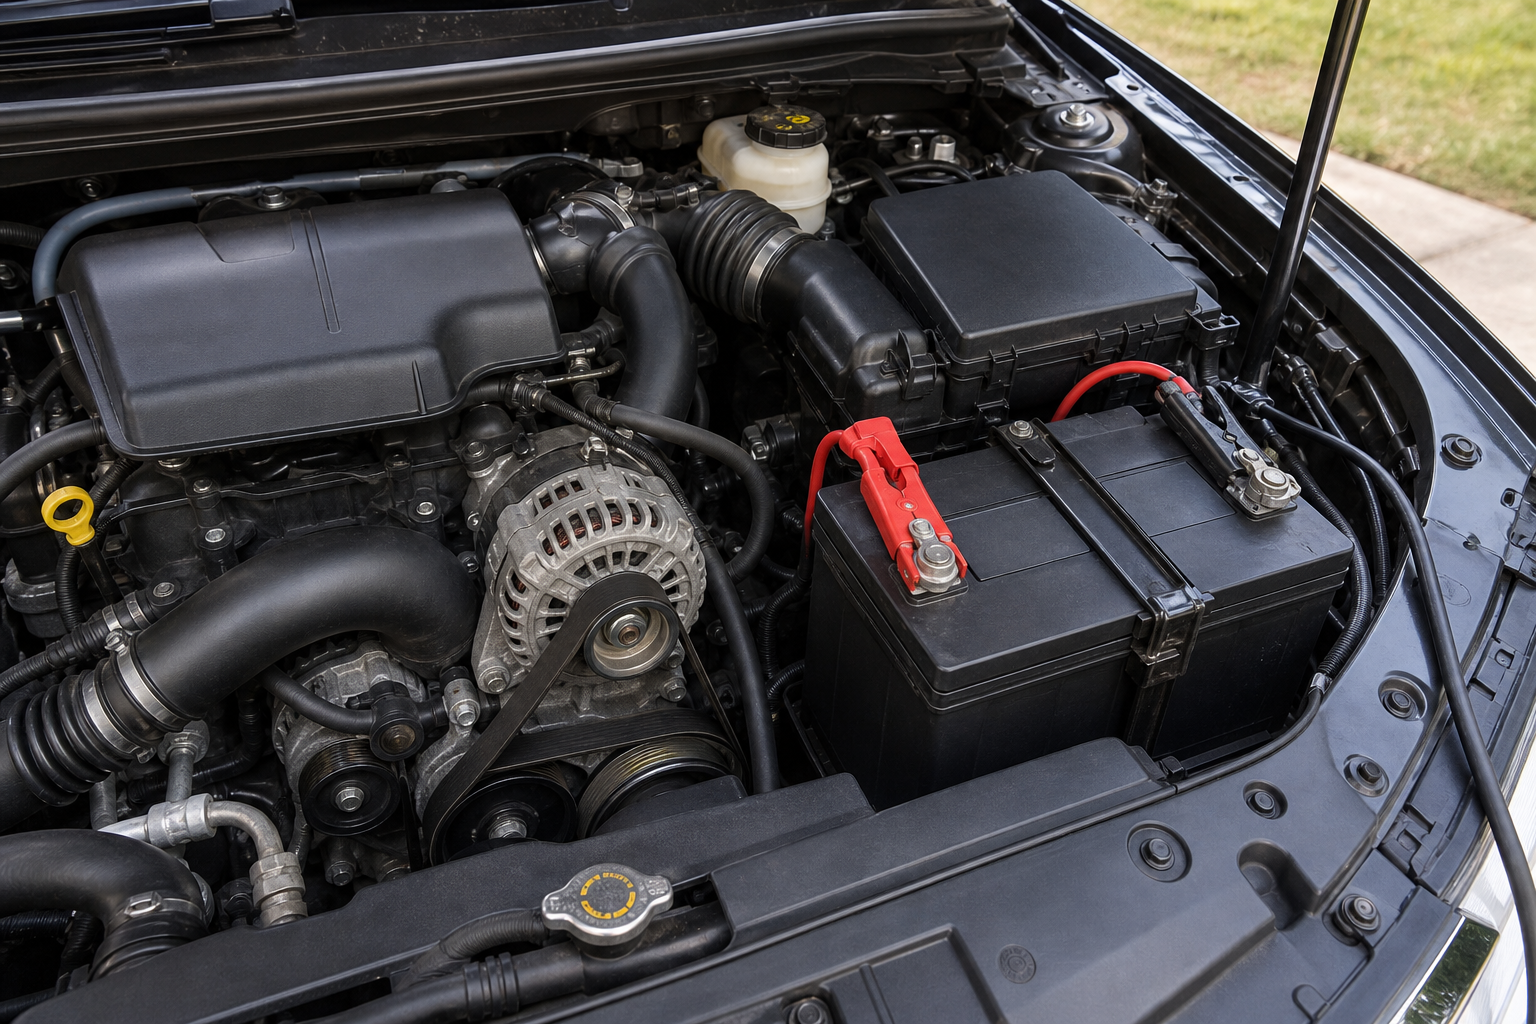
\includegraphics[width=0.58\linewidth]{images/book3/ai/b3-06-car-battery-engine-bay.png}

{\small Di bawah kap mesin: aki \qty{12}{V}, kabel tebalnya dan alternatornya --- jaringan arus searah pada soal akhir pekan, dengan ratusan \omterm{def:b1:dc-circuits:current}{ampere} pada saat menghidupkan mesin.}
\end{omfigure}

\section{Soal: Sistem kelistrikan sebuah mobil}

\begin{problem}[{Soal akhir pekan --- satu aki, sebuah starter, dua
lampu depan, sebuah alternator dan beberapa meter tembaga: siapa yang
mendapat arusnya, siapa yang membayarnya, dan mengapa lampunya meredup
ketika mesinnya diengkol}]
\label{pb:b1:dc-circuits:1}
Akinya adalah sumber nyata, ggl $E = \qty{12.6}{V}$, \omterm{def:b1:dc-circuits:sources}{hambatan dalam}
$r = \qty{10}{m\ohm}$. Tembaga: $\rho = \qty{1.7e-8}{\ohm.m}$.

\medskip
\noindent\textbf{Bagian I --- Akinya sendirian.}
\begin{enumerate}
  \item Lukislah \omterm{def:b1:dc-circuits:sources}{model Thévenin} lalu tuliskan $u(i)$ dalam \omterm{thm:b1:dc-circuits:kirchhoff}{kesepakatan
        pembangkit}.
  \item Berikan \omterm{def:b1:dc-circuits:voltage}{tegangan} rangkaian terbukanya dan arus hubung
        singkatnya. Mengapa kunci pas yang terjatuh tak boleh
        menjembatani kutubnya?
  \item Tuliskan \omterm{def:b1:dc-circuits:sources}{model Norton} aki yang sama.
  \item Akinya memberi daya kepada \omterm{def:b1:dc-circuits:resistor}{resistor} $R$: nyatakan arusnya,
        \omterm{def:b1:dc-circuits:voltage}{tegangan} pada ujungnya, daya $P_R$ yang diberikan dan daya yang
        hilang di $r$.
  \item Tunjukkan bahwa $P_R$ maksimum untuk $R = r$ lalu hitunglah
        maksimum itu. Berapa efisiensinya ketika itu?
  \item Seorang teknisi mengukur $u = \qty{12.48}{V}$ pada \qty{12}{A}
        dan $u = \qty{11.40}{V}$ pada \qty{120}{A}. Periksalah bahwa
        kedua titiknya terletak pada modelnya lalu jelaskan bagaimana
        deretan titik semacam itu memberi $E$ dan $r$ lewat pencocokan
        garis lurus.
  \item Akinya menyimpan \qty{60}{A.h}. Berapa lama ia dapat menyalakan
        kedua lampu depan \qty{55}{W} itu sendirian (ambil \qty{12}{V})?
        Berapa besar energinya dalam joule?
\end{enumerate}

\medskip
\noindent\textbf{Bagian II --- Mengengkol dengan lampu menyala.}
Starternya adalah \omterm{def:b1:dc-circuits:resistor}{resistor} $R_s = \qty{80}{m\ohm}$; tiap lampu depan
berdaya \qty{55}{W} pada \qty{12.0}{V} dan diperlakukan sebagai \omterm{def:b1:dc-circuits:resistor}{resistor}.
\begin{enumerate}[resume]
  \item Hitunglah hambatan satu lampu depan dan hambatan keduanya ketika
        terangkai paralel.
  \item Starter sendirian: arusnya, \omterm{def:b1:dc-circuits:voltage}{tegangan} pada ujungnya, daya pada
        starternya, dan daya yang hilang di akinya.
  \item Starter dan kedua lampu depan bersama-sama: hambatan beban
        setaranya, arus totalnya, \omterm{def:b1:dc-circuits:voltage}{tegangan} pada ujungnya.
  \item Pakailah \omterm{prop:b1:dc-circuits:dividers}{pembagi arus} untuk mencari arus starternya dan arus
        lampu depannya.
  \item Hitunglah daya yang kini diterima tiap lampu depan lalu
        bandingkan dengan dayanya yang tertera: seberapa besar bagian
        lampunya meredup?
  \item Jelaskan dalam dua kalimat, dengan memakai \omterm{thm:b1:dc-circuits:kirchhoff}{hukum loop}, mengapa
        lampunya meredup justru karena starternya menarik arus yang besar.
  \item Apakah kabel aki yang lebih tebal akan menolong lampunya?
        Berikan alasan kualitatif sekarang (Bagian IV menghitungnya).
\end{enumerate}

\medskip
\noindent\textbf{Bagian III --- Mesin hidup: alternatornya.}
Alternatornya adalah sumber nyata kedua, $E_a = \qty{14.2}{V}$,
$r_a = \qty{50}{m\ohm}$, yang terangkai paralel dengan akinya; starternya
mati dan kedua lampu depannya menyala.
\begin{enumerate}[resume]
  \item Lukislah rangkaiannya: dua sumber nyata dan beban lampu depannya
        terangkai paralel di antara dua simpul yang sama.
  \item Terapkan teorema Millman untuk mencari \omterm{def:b1:dc-circuits:voltage}{tegangan} bersama pada ujungnya.
  \item Simpulkan arus alternatornya, arus akinya (perhatikan tandanya)
        dan arus lampu depannya; periksalah \omterm{thm:b1:dc-circuits:kirchhoff}{hukum simpulnya}.
  \item Apakah akinya sedang diisi atau sedang mengosong? Berapa daya
        yang diterimanya, dan berapa daya yang dipasok alternatornya?
  \item Perolehlah kembali \omterm{def:b1:dc-circuits:voltage}{tegangan} pada ujungnya lewat superposisi
        (tiap sumber sendirian, yang lain diganti \omterm{def:b1:dc-circuits:sources}{hambatan dalamnya})
        lalu periksalah.
\end{enumerate}

\medskip
\noindent\textbf{Bagian IV --- Sensor dan kawat.}
\begin{enumerate}[resume]
  \item Sensor pendinginnya adalah termistor yang hambatannya turun dari
        \qty{2.0}{k\ohm} pada \qty{20}{\degreeCelsius} ke \qty{300}{\ohm} pada
        \qty{90}{\degreeCelsius}; ia menjadi \omterm{def:b1:dc-circuits:resistor}{resistor} bawah sebuah pembagi
        yang diberi \qty{5.0}{V}, dengan \omterm{def:b1:dc-circuits:resistor}{resistor} atasnya $R_0$. Nyatakan
        \omterm{def:b1:dc-circuits:voltage}{tegangan} keluarannya, lalu hitunglah pada kedua suhu itu untuk
        $R_0 = \qty{775}{\ohm}$.
  \item Tunjukkan bahwa ayunan keluaran antara kedua suhu itu paling
        besar ketika $R_0$ merupakan rata-rata geometri kedua nilai
        sensornya, lalu periksalah nilai di atas.
  \item Sensor yang sama dipasang dalam \omterm{prop:b1:dc-circuits:wheatstone}{jembatan Wheatstone} bersama tiga
        \omterm{def:b1:dc-circuits:resistor}{resistor} \qty{775}{\ohm}: tuliskan keluaran jembatannya lalu
        katakan pada suhu berapa ia setimbang.
  \item Kabel starternya sepanjang \qty{1.5}{m} untuk tiap arah.
        Hitunglah hambatan satu penghantar berpenampang \qty{16}{mm^2},
        jatuh \omterm{def:b1:dc-circuits:voltage}{tegangan} totalnya pada \qty{140}{A}, dan daya yang
        dilesapkan di kabelnya.
  \item Sama untuk kabel \qty{4}{mm^2}: mengapa kabel starter setebal itu?
  \item Ringkaslah: berikan \omterm{def:b1:dc-circuits:voltage}{tegangan} pada ujungnya selama pengengkolan,
        bagian daya yang mencapai starternya, dan satu hukum yang
        menjelaskan meredupnya lampu.
\end{enumerate}
\end{problem}
